In order to complete the work required to meet my aims, various pieces of software, tools and methods are required. Appropriate (spatially-aware) relational database software is chosen and developed to store and interrogate data, geographic information systems (GIS) and statistical programming languages are used for spatial data processing and visualisation, statistics software for drawing conclusions from the processed data, and other libraries and software such as CartoDB and D3 javacript are used for visualisation and presentation.

The tools and methods I have chose to work with are all 'Free and Open Source Software' (FOSS) rather than commercial or proprietary alternatives. This choice is mostly made as it is the author’s belief that community developed software leads to easier and readily available customisation by the users, more frequent improvements and updates, quicker fixing of bugs, and generally more choice of tools for specific purposes. Given the software is free, this also negates any concerns about licenses and installation on multiple computers which might be a concern with other software.

%%%%%%%%%%%%%%%%%%%%%%%%%%%%%%%%%%%
%%% The LTDS
%%%%%%%%%%%%%%%%%%%%%%%%%%%%%%%%%%%

\section{The London Transport Demand Survey}
\label{sec:the_ltds}

The London Transport Demand Survey (The LTDS) is a survey of households in the London area, covering all London Borough's as well as the area between those Borough's and the M25. It is organised by the Strategic Analysis section of the Planning department at Transport for London. The survey is a continuous rolling--survey, started in 2005--2006, and still happening today. Around 8,000 households per year are surveyed.

The LTDS survey captures information on households, the people that live in those households, the trips that those people make in the day, and the vehicles that they use/own. Everyone in the house that is surveyed answers the questionnaires, except for children under the age of 5. There are three questionnaire that each person completes. The household questionnaire gives details on household structure and includes demographic information such as income, housing tenure and vehicle ownership. The individual questionnaire contains demographic information about the individuals in the household, working status, frequency of transport mode use, driving licenses, public transport tickets held and similar. The third questionnaire is the trip sheet which is key to how I will use this data. It captures data on all the trips made on the designated travel day (which is the same day for all members of the household). The details include the purpose of the trip, the transport modes that were used, the time of the day the trip started, the time of the day the trip ended, and the origin and destination of the trips. This section of the database can effectively be used to interrogate exactly where each person was during the 24 hours that the survey covers (it covers 4am on the day of the survey, to 4am on the following day, unless that person was in-transit at 4am in which case it continues until the journey is complete).

The LTDS is designed to enable statistically-robust representative estimates of travel patterns and demand in London. Results from a single year are robust enough to analyse at the London-wide level, however combining three or more years data for analysis is preferable. The results can be considered at a London-wide level, or disaggregated to Borough of residence.

The database contains 100 tables of data, however many of these are 'look-up' tables for data in the main tables. For example the year that a household was surveyed is stored in a column called 'hyearid' which simply contains a number between 5 and 9. These numbers allow linkage to a table called YEARID\_T where the value 5 can be seen to correspond to the description of '2005/2006'. A summary of the key tables and numbers of records in these tables of the LTDS that I use is shown below in Table \ref{tab:ltds_data}.

\begin{table}[H]
    \begin{tabular}{ | p{2.2cm} | p{2.2cm} | p{2.2cm} | p{2.2cm} | p{2.2cm} |}
    \hline
    \textbf{Year} & \textbf{Households} & \textbf{People} & \textbf{Trips} & \textbf{Stages} \\ \hline
    2005--2006 & 5,008 & 11,583 & 29,797 & 61,542 \\ \hline
    2006--2007 & 8,005 & 18,241 & 47,029 & 95,930 \\ \hline
    2007--2008 & 7,873 & 17,926 & 44,828 & 91,967 \\ \hline
    2008--2009 & 8,134 & 18,975 & 43,076 & 89,701 \\ \hline
    2009--2010 & 8,290 & 19,187 & 43,475 & 92,121 \\ \hline
    \end{tabular}
    \caption{Data contained in the LTDS}
    \label{tab:ltds_data}
\end{table}

%%%%%%%%%%%%%%%%%%%%%%%%%%%%%%%%%%%
%%% Spatial databases
%%%%%%%%%%%%%%%%%%%%%%%%%%%%%%%%%%%

\section{Spatial databases}
\label{sec:spatialdatabases}

Relational database management systems (RDMS) are a common tool and are widely used for effectively storing and querying datasets. However to meet my research aims a RDMS that can store extensive spatial and temporal data was needed, and these are much less common. Spatially aware databases have been developed alongside GIS systems and are traditionally seen as the back-end of a GIS i.e. the place where the data is stored, while the GIS serves it to the user in a graphical map-like interface where a user might do analysis. However as spatially-aware databases have become more common, a disconnect has occurred and now it is not uncommon to use spatial databases on their own, and only connect them to a GIS when needed (if at all).

The specifications of what a spatial database should be were published in the very highly cited (884 at time of writing) 1994 paper \textit{'An introduction to spatial database systems}'. This paper is so well cited as it was the first paper to really define what a spatial database was, namely '\textit{a database system that offers spatial data types in its data model and query language and supports spatial data types in its implementation, providing at least spatial indexing and spatial join methods}' (\cite{Guting1994}). More recently \cite{ObeHsu201410} defined it as a \textit{a database that defines special data types for geometric objects and allows you to store geometric data (usually of a geographic nature) in regular database tables. It provides special functions and indexes for querying and manipulating that data using something like Structured Query Language (SQL)}.

There are a selection of spatial databases which could be used for the storage of the data required for this work. \cite{Ellul2012} identifies the three most popular spatial-RDMS as:

\begin{itemize}
\item PostgreSQL (\cite{PostgreSQL2014})
\item Oracle Express (\cite{Oracle2014})
\item MySQL (\cite{MySQL2014})
\end{itemize}

Of these three, I chose PostgreSQL (with the spatial add-on PostGIS) for this research due to it's ease of installation on multiple operating systems, but more importantly for the greater availability of spatial SQL queries when compared to the other two systems. That is, more functions and tools for manipulating spatial data are available in this system than in the other two alternatives. The range of FOSS desktop GIS that can easily be connected to PostGIS was also a consideration, as was (to a lesser degree) my familiarity with their use. Relevant data from the LTDS (described in Section \ref{sec:the_ltds}) is therefore exported from the Access database from in which it was provided by TfL, and uploaded to PostgreSQL instead.

%%%%%%%%%%%%%%%%%%%%%%%%%%%%%%%%%%%
%%% GIS
%%%%%%%%%%%%%%%%%%%%%%%%%%%%%%%%%%%

\section{Geographic Information Systems \& Science (GIS)}
\label{sec:gis}

FOSS that is specifically used for geographic type data, such as a GIS, is often referred to as FOSS4G (Free and Open Source Software for GIS/Geospatial). Different categories of GIS are designed for different purposes. Each GIS product, whether web-based, desktop client or otherwise tends to perform a number of functions. \cite{Steiniger2013} summarises the functions as follows:

\begin{enumerate}
\item Data creation
\item Data editing
\item Data storage
\item Data integration
\item Data querying
\item Data analysis
\item Data transformation
\item Map creation
\item Data visualisation 
\end{enumerate}

It is typical to use a desktop-based client for the majority of the uses listed above, but as I decided to use the PostgreSQL \& PostGIS RDMS (see section \ref{sec:spatialdatabases}) for items 1-8 of the list, the full functionality of a typical GIS is not required, as the GIS is mostly just used for map creation after processing of the data within the database itself. This approach is taken as keeping the data within the database until it is ready for visualisation leads to quicker processing and manipulation of the data.

Maps are normally defined either as static maps or dynamic/slippy maps. A static map being a map that is produced using a GIS Desktop client and then outputted as a PDF or PNG file or similar, and then perhaps embedded in a document or presentation. Once produced the data cannot be edited by the viewer, or the area of the map changed. For this type of output, I use the Quantum GIS (QGIS) (\cite{qgis2014}) project. QGIS is a user-friendly Open Source GIS, licensed under the GNU General Public License. It is developed by the Open Source Geospatial Foundation (OSGeo) and runs on Linux, Unix, Mac OSX, Windows and Android. It supports numerous vector, raster, and database formats and functionalities. QGIS is the most popular, comprehensive and stable FOSS4G software and so was the obvious choice.

%%%%%%%%%%%%%%%%%%%%%%%%%%%%%%%%%%%
%%% Routing
%%%%%%%%%%%%%%%%%%%%%%%%%%%%%%%%%%%

\section{Routing}
\label{sec:routing}

One of the innovative aspects of this research is to attempt to quantify exposure across space and time, rather than in static locations such as homes and offices. In order for this to be possible, data on the subjects locations on a fine temporal and spatial resolution is required. The data provided by TfL and included in the LTDS database gives geographical and temporal data (as well as mode of travel) on the start and end locations of journeys that the subjects make, but not the routes that the journey took. To calculate this missing information routing databases and Application Programming Interfaces (APIs) can be used. By doing so routes between two points that respect the road/cycle/train etc networks will be generated and stored, rather than perhaps drawing a straight line between the two locations. 
To use a routing database network data on the choice of transport mode is required and then requests need to be made to this network for routes using SQL queries. 

Loading of these network datasets can be accomplished by downloading the data, for example from OpenStreetMap, and then processing and importing it into PostgreSQL. Once this is done, the FOSS PostgreSQL add-on pgRouting is installed and the network data is processed and a topology of the network is created which is suitable for use with standard SQL query language. The benefits of this approach are that the network is in complete control of the user and can be customised at will, for example road speed-limits can be adjusted (which will affect routes chosen by the algorithms), a preference for certain road types factored in, one-way restrictions either ignored or obeyed. There is also a certain independence to this approach i.e. no reliance on an external provider keeping the dataset up-to-date or needing a web connection for the routing to take place (as is required for the API approach discussed shortly). On the negative side however the network can be difficult and time-consuming to set-up in the first place, the amount of data to download and process is large and complex, and a new network is required for each transport mode that routing will be required for. This is particularly pertinent for the LTDS as routing on many different transport modes is required including underground, bus, cycling, driving, walking and overground/mainline trains - and data to create networks for each of these modes is difficult to obtain and maintain, particularly for bus routes and train lines as the data is held by the relevant companies that operate these services and even when made publicly available is often not in a suitable format or there is missing information.

APIs offer an alternative approach to routing. Instead of building and maintaining network datasets in a users own database/server, the networks are hosted by other commercial and non-commercial organisations who allow external users to interact with their data (but not to edit it or use it in ways which they do not allow).  A user, having read the normally provided documentation, first forms a query string (similar to a website address but longer and more complex) and then 'sends' this to the organisations API service. The API interprets the request that the user has made, and 'returns' the data required. In the case of routing, the request from the user is typically a start-point, end-point, transport mode and time of travel, and the return from the API is a route made up of such information as a list of tube stations, or coordinates, or text instructions. The amount of detail that can be submitted as a request, and the amount of detail that is provided by the reply, varies by service. A typical request string to the TfL directions API is shown in figure \ref{fig:tfl_api_call}.

\begin{figure}[H]
\centering
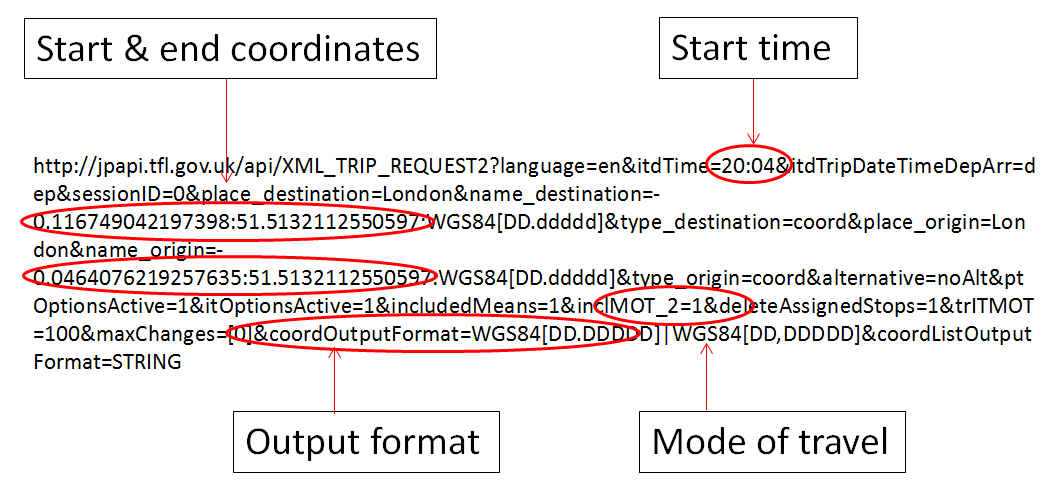
\includegraphics[scale=0.5]{tfl_api_call}
\caption{A 'call' to the TfL routing API}
\label{fig:tfl_api_call}
\end{figure}

This is submitted to the API using software of the users choice, code is written to parse the data that is returned (made into a format that the software can read), and then the results are stored and used as the user wishes.

A search of routing API services was therefore conducted, based upon the list detailed in the Wikipedia page 'Online Routers' (\url{http://wiki.openstreetmap.org/wiki/Routing/online_routers}) as well as an internet search of the term 'Online routing API'. A review of those considered suitable for this research is presented in table \ref{tab:api_summary_table}. A small handful of other APIs were dismissed before this stage as they were unsuitable for reasons such as geography (e.g. only covers Germany) or the API does not expose the route to the user (e.g. Bing Maps Directions plots the line onto a map, but does not give the actual data for storage).

\begin{landscape}
\begin{table}
    \hspace*{-.1cm}%
    \begin{tabular}{@{}| R{3.3cm} | R{3.2cm} | R{1.9cm} | R{3.2cm} | R{3.4cm} | R{4.5cm} |@{}}

    \hline

\textbf{API Service (coverage)} & \textbf{Available transport modes} & \textbf{Usage limits} & \textbf{Documentation} & \textbf{Simplicity of use} & \textbf{Customisation and notes} \\ \hline

Google Directions API (Worldwide) & Car, pedestrian, cycling, public transport & 750 per day (without license) & Provided, with many examples & Very simple to use & Limited. Parameters such as use of tolls, language of content, shortest or quickest. Public transport modes cannot be distinguished \\ \hline

OpenRouteService (Worldwide, but dependant on OSM data quality) & Car, pedestrian, cycling & Unlimited & In the form of a Wikipedia entry. Covers some examples but is not comprehensive. & Very simple & Limited. Road types, languages, zoom levels \\ \hline

Project OSRM (Open Source Routing Machine) (Worldwide, but dependant on OSM data quality) & Car & Unlimited & Basic instructions provided on GitHub & Very simple to use & Limited. Zoom level and output file type \\ \hline

Transport for London (Greater London) & Underground, overground, bus, train, tram, boat, cable---car, Docklands Light Railway & Unlimited (once registered) & Extremely comprehensive manual, but unclear in many places and often seemingly contradictory & Very difficult. Only simple examples are provided. So many parameters must be considered for a properly formed request & Fully customisable in almost every way. However it is limited to Greater London and does not alert when routes go outside. \\ \hline

MapQuest (Worldwide) & Car & Unlimited & Basic instructions provided on GitHub & Very simple to use & Limited. Zoom level and output file type \\ \hline

\end{tabular}\hspace*{-2cm}%%stop complaining
\caption{Summary of suitable routing APIs}
\label{tab:api_summary_table}
\vspace{-1cm}%%stop complaining
\end{table}
\end{landscape}

Each routing tool has advantages and disadvantages and it is therefore my expectation that a combination of these will need to be used depending on the specific use-case e.g. routes using the London Underground will need to use the TfL API.

%%%%%%%%%%%%%%%%%%%%%%%%%%%%%%%%%%%
%%% CMAQ-Urban
%%%%%%%%%%%%%%%%%%%%%%%%%%%%%%%%%%%

\section{CMAQ Urban}
\label{sec:cmaq_urban}

CMAQ (Community Multi-scale Air Quality model) is an ongoing open-source project, coordinated/led by the U.S. EPA Atmospheric Science Modelling Division. It is made up of a variety of software packages and processes for simulating air quality. To quote from their website, "CMAQ combines current knowledge in atmospheric science and air quality modeling with multi-processor computing techniques in an open-source framework to deliver fast, technically sound estimates of ozone, particulates, toxics, and acid deposition" (\cite{UnitedStatesEnvironmentalProtectionAgency2014}). The three main components are as follows (\cite{CMASCentre}):

\begin{enumerate}
\item A meteorological modelling system for the description of atmospheric states and motions
\item Emission models for man-made and natural emissions that are injected into the atmosphere
\item A chemistry-transport modelling system for simulation of the chemical transformation and fate
\end{enumerate}

ADMS-Urban is a separate air quality model which is distinctive as it is able to model a range of scales, from street to city, taking into account emissions sources such as traffic, industry and domestic sources. It incorporates advanced algorithms for the height-dependence of wind-speed, turbulence and stability to produce predictions. It also includes information on street canyons and mixing introduced by road traffic re-suspension  (\cite{CambridgeEnvironmentalResearchCounsultantsCERC2014a}).

The Environmental Research Group at King's College London, where the research within this report is taking place, have created a version of ADMS-Urban (KCL-Urban) which gives annual mean air quality predictions of NO, NO$_{2}$, O$_{3}$, PM$_{10}$ and PM$_{2.5}$ on a regular 20 m x 20 m grid. This is combined with a CMAQ regional scale model to create CMAQ-Urban which provides predictions of the same pollutants at the same scale on an hourly temporal resolution. The two models are equipped with similar capabilities in that KCL-Urban is quick to run and can provide details of the poor air quality sources at any location within it's domain. By combining these two ( CMAQ and KCL-Urban) the result is a model which is partly deterministic (uses fundamental physics and chemistry), but provides the same spatial detail as KCL-Urban. Importantly, it is therefore capable of predicting hourly concentrations (\cite{Beevers2013}). An example of the output of CMAQ-Urban is shown in Figures \ref{fig:kcl_urban_no2} and \ref{fig:cmaq_uk}.

\begin{figure}[H]
\centering
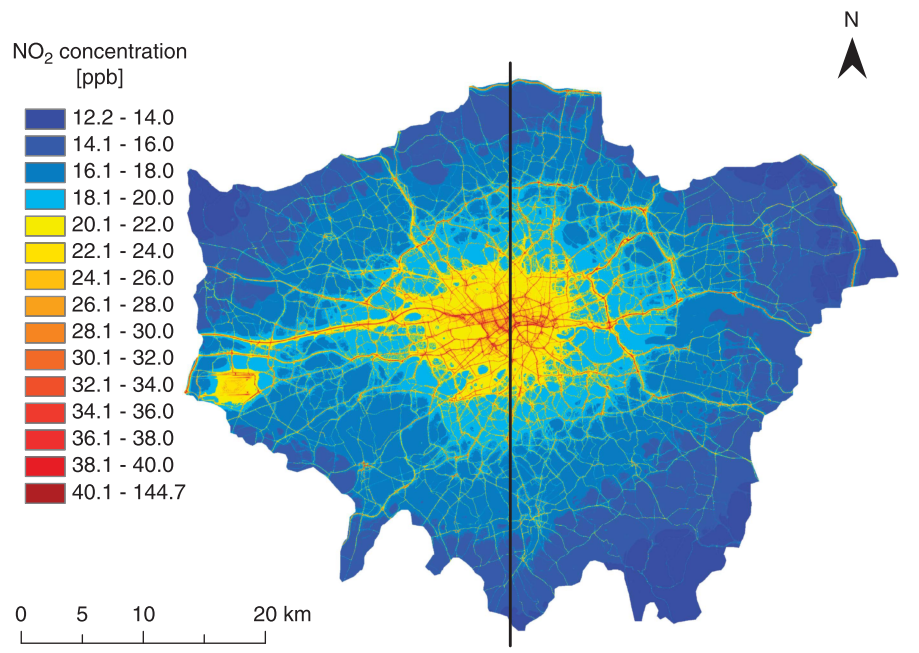
\includegraphics[scale=0.6]{kcl_urban_no2}
\caption{Annual mean NO$_{2}$ concentrations in London for the year 2008 predicted onto a regular grid of 20 m x 20 m using the KCLurban model.}
\label{fig:kcl_urban_no2}
\end{figure}

\begin{figure}[H]
\centering
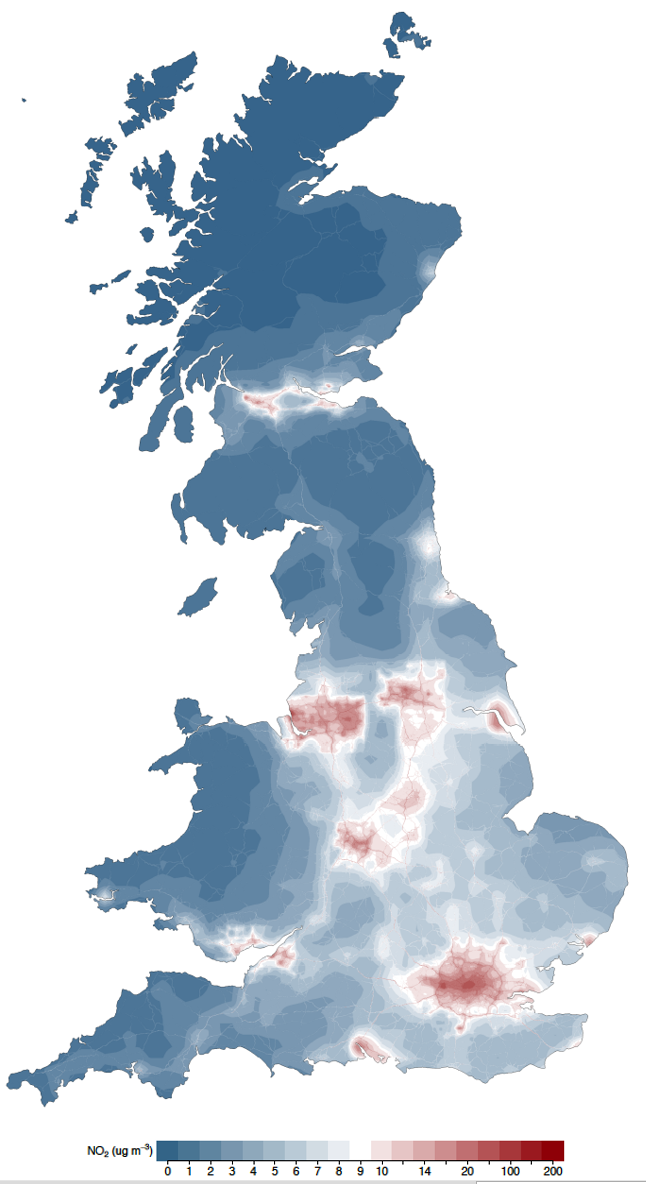
\includegraphics[scale=0.8]{cmaq_uk_v2}
\caption{An illustrative example of the domain covered by CMAQ-Urban}
\label{fig:cmaq_uk}
\end{figure}

CMAQ-urban was submitted to the  UK Model Intercomparison exercise run by the UK Government department DEFRA (\cite{Carslaw2013}), where it performed well against other urban and regional models with r values of 0.9 for NO$_{X}$ and NO$_{2}$, and 0.77 for PM$_{2.5}$.

For calculating exposure on a fine temporal (monthly-daily-hourly averages) and spatial scale (20 m x 20 m grids) the locations and time of individual subjects will be spatially joined with this model and then concentrations extracted from it.

%%%%%%%%%%%%%%%%%%%%%%%%%%%%%%%%%%%
%%% Interactive data visualisations
%%%%%%%%%%%%%%%%%%%%%%%%%%%%%%%%%%%

\section{Interactive data visualisations and animations}
\label{sec:interactivedata}

When it is desirable to produce maps of a higher quality, perhaps with interactive elements such as the user being able to click for more details or zoom in on areas of interest, the static maps that QGIS can produce as a PDF or similar are not suitable, and different tools are used to produce slippy maps (maps that can be dragged around using a mouse or other input device) with overlays of data. Figure \ref{fig:clear_streets} shows the website \url{www.clearstreet.org} which uses such a 'slippy' map and allows the viewer to zoom in or out on their area and examine the snow-plough activity.

\begin{figure}[H]
\centering
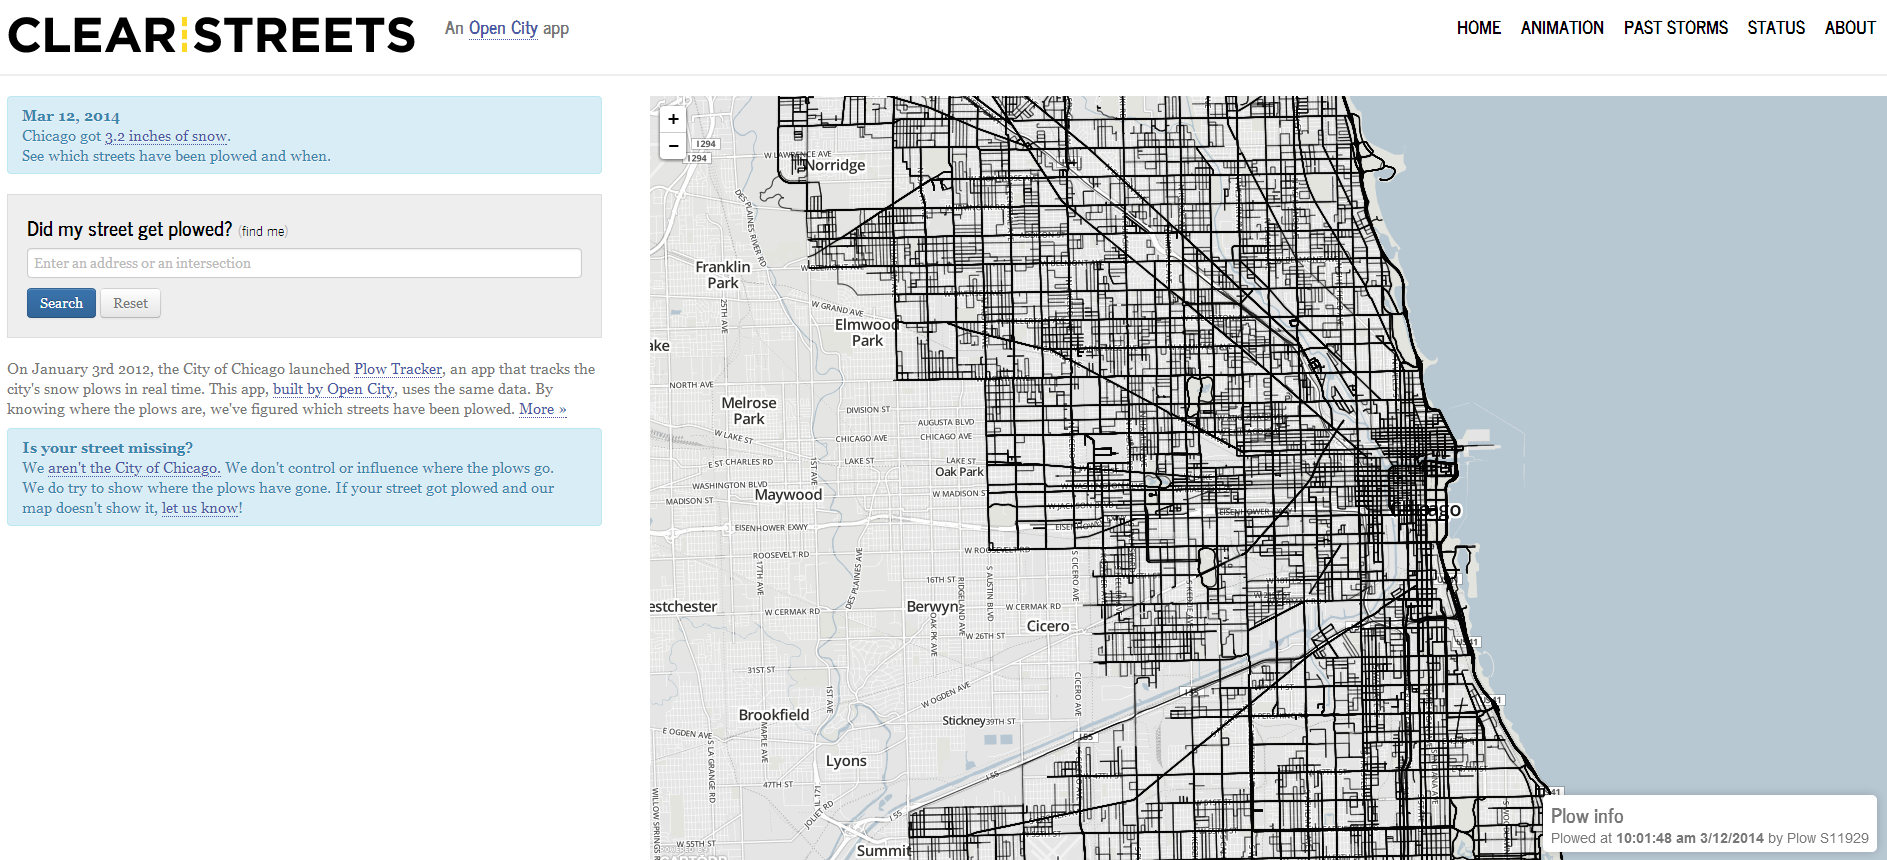
\includegraphics[scale=0.3]{clear_streets}
\caption{The clear streets website with a 'slippy' map}
\label{fig:clear_streets}
\end{figure}

Previously making maps of this type required specialist GIS and programming skills, and were almost exclusively made using the Google Maps API which allows embedding of the Google Maps data on your own webpage and with your own data added, however there has been a huge surge in mapping products over the last five to ten years as the profitability and usage of geographical data has become clear and commonplace respectively. As the field is rapidly evolving most books or review articles are out-of-date within weeks of publication, and therefore the following list of providers of global web-based slippy maps is taken from Wikipedia (\cite{wiki-maps-2014}):

\begin{itemize}
\item OpenStreetMap  (\url{http://www.openstreetmap.org/})
\item ArcGIS Online (Esri)  (\url{http://www.arcgis.com/home/webmap})
\item Google Maps \url{https://www.google.com/maps/})
\item Bing Maps (\url{http://www.bing.com/maps/})
\item MapQuest (\url{http://www.mapquest.com/})
\item WikiMapia (\url{http://wikimapia.org/})
\item HERE (\url{http://here.com/})
\item Mappy (\url{http://en.mappy.com/})
\item Yahoo! Maps (\url{https://maps.yahoo.com/})
\end{itemize}

Of this list the most popular and widely used are Google Maps and OpenStreetMap, however in following with the earlier stated aim of using FOSS tools, I decided to use OpenStreetMap background data for making online maps where needed in this research, due to it's community-made nature and lack of any restrictions on it's use or frequency of use.

To be able to use OpenStreetMap data as a background map with overlaps of data that has been produced during this research, further tools are needed. The two introduced below are both FOSS4G implementations of the javascript programming language and I intend to use them both as required, particularly for the later in this research where I explore novel visualisations and techniques for exposure and air quality data. 

\begin{itemize}
\item CartoDB.com (figure \ref{fig:cartodb_screen}): CartoDB is a cloud-based web-mapping, analysis and visualisation service. It allows storage of geographical data on their servers which can then be visualised on a map and published to a webpage. The advantages of CartoDB are the simplicity of producing professional looking maps with very little effort, however the amount of data that can be stored is limited without having to pay for additional storage. Despite this, for ad-hoc visualisations and/or ones that do not require a large amount of data to be displayed, this tool is very useful. CartoDB.com uses OpenStreetMap data as the background for the maps that it serves to the users and can be easily customised.
\item Leaflet.js: Leaflet prides itself as a lightweight javascript library which displays OpenStreetMap data. By lightweight the community developers emphasise the very small amount of coding and expertise that is required to produce a map. Adding data and creating visualisations on top of the map is then of moderate difficulty. The main difference between CartoDB and Leaflet is that leaflet does not store the data, the webpage is coded so that the data is fed to it from another source such as an API or indeed a CSV file or similar which is stored on the same server as the map-coding itself. This has the advantage of there being no data-storage limits as the developer is responsible for the data themselves, however the knowledge and skills required to put the data onto the map are more advanced than that of using CartoDB.
\end{itemize}

\begin{figure}[H]
\centering
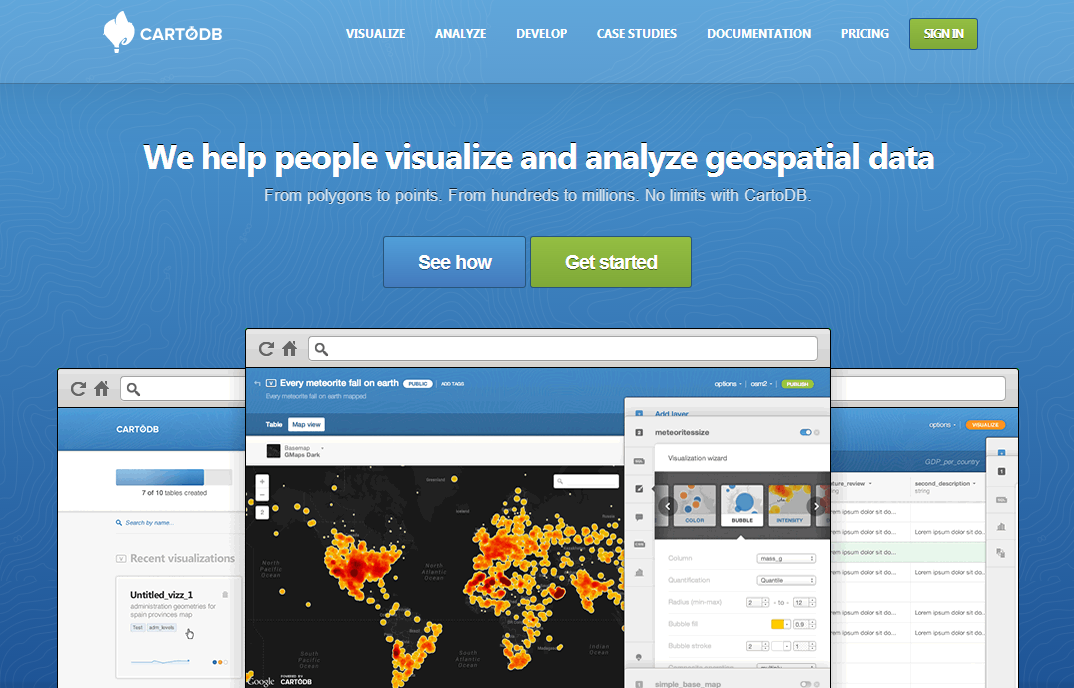
\includegraphics[scale=0.5]{cartodb_screen}
\caption{The CartoDB data visualisation platform}
\label{fig:cartodb_screen}
\end{figure}

When outputs of this research are required that are not suitable for a map, then I will make graphs and charts using the plotting functionality of the FOSS 'R' project (\cite{RFoundationforStatisticalComputing2014}). One of the benefits of using R is that it can be easily connected to the PostgreSQL RDMS that was chosen earlier, and then statistical analysis and publication-quality plots can be produced with relative ease and a few lines of coding.  For interactive or web-based charts and graphs the D3 javascript library developed by Mike Bostock will instead be used (\cite{Bostock:2011:DDD:2068462.2068631}) for similar reasons - it is free, open-source, and there is a large community of developers actively using it which gives a great deal of inspiration and examples to base future work on e.g. \url{https://github.com/mbostock/d3/wiki/Gallery}.